\documentclass[tikz,border=3mm]{standalone}
\usepackage[utf8]{inputenc}
\usepackage[T1]{fontenc}
\usepackage{helvet}
\renewcommand{\familydefault}{\sfdefault}
\usetikzlibrary{arrows.meta,positioning}
\begin{document}

\tikzset{every node/.append style={font=\sffamily\small}}
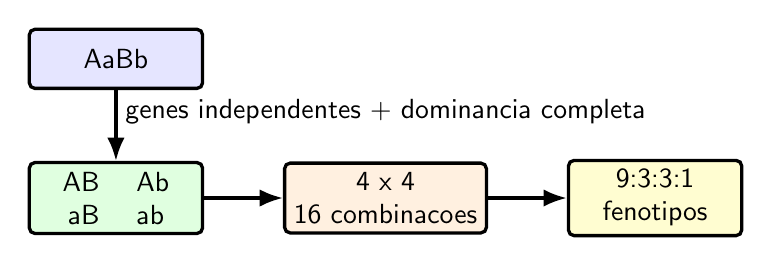
\begin{tikzpicture}[>=Latex,node distance=0.75cm]
  \tikzstyle{box}=[draw,rounded corners=2pt,very thick,align=center,minimum width=2.2cm,minimum height=0.75cm]
  \node[box,fill=blue!10] (aabb) {AaBb};
  \node[box,fill=green!12,below=0.9cm of aabb] (gam) {AB \quad Ab\\aB \quad ab};
  \node[box,fill=orange!12,right=1.0cm of gam] (pun) {4 x 4\\16 combinacoes};
  \node[box,fill=yellow!18,right=1.0cm of pun] (prop) {9:3:3:1\\fenotipos};
  \draw[very thick,->] (aabb) -- (gam);
  \draw[very thick,->] (gam) -- (pun);
  \draw[very thick,->] (pun) -- (prop);
  \node[align=center,above=0.35cm of pun] {genes independentes + dominancia completa};
\end{tikzpicture}
\end{document}
